209. \begin{figure}[ht!]
\center{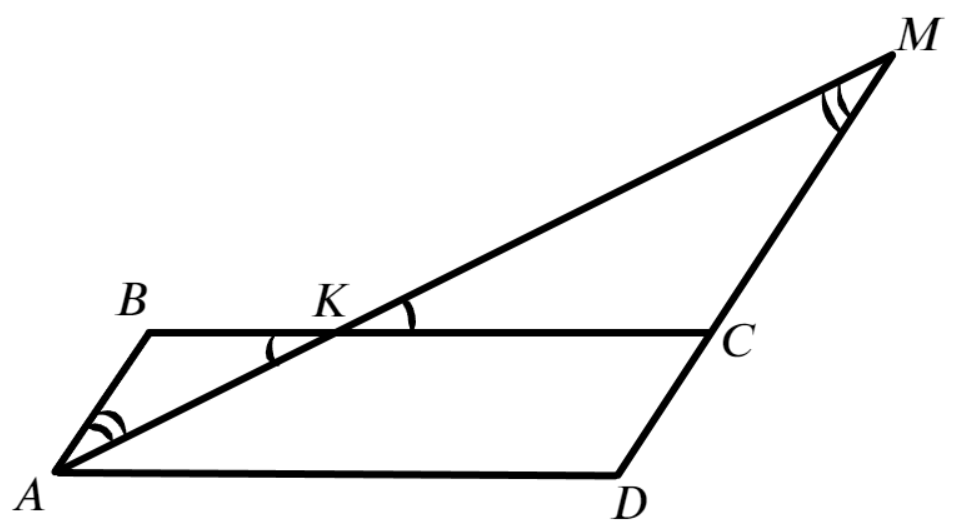
\includegraphics[scale=0.35]{g8-209.png}}
\end{figure}\\
$\angle BAK=\angle KMC$ как накрест лежащие, а $\angle AKB=\angle CKM$ как вертикальные. Тогда треугольники $ABK$ и $MCK$ подобны по двум углам и $\cfrac{KC}{BK}=\cfrac{CM}{AM}=\cfrac{DM-DC}{DC}=\cfrac{3DC-DC}{DC}=2.$ Поэтому $\cfrac{BC}{BK}=\cfrac{BK+KC}{BK}=1+2=3.$ Если опустить высоту $h$ из точки $A$ на $BC,$ то $\cfrac{S_{ABCD}}{S_{\Delta ABK}}=\cfrac{h\cdot BC}{\cfrac{1}{2}h\cdot BK}=2\cdot3=6.$ Таким образом, $S_{\Delta ABK}=S_{ABCD}:6=12:6=2.$\\
